\documentclass{beamer}
\mode<presentation>
{
  \usetheme[height=40pt]{ScarletHannover} %UNL-Sbaush, MyHannover, BlueHannover, ScarletHannover, Lart
  \useinnertheme[shadow=true]{rounded}
  %\useoutertheme{shadow}  
   \usefonttheme{professionalfonts}
  %\usefonttheme{structureitalicserif,structuresmallcapsserif,professionalfonts,serif,structurebold,}
   
   %\usecolortheme{sbaushOUTER} % ---> OUTER
   %\usecolortheme{sbaushINNER} % ---> INNER
   %\usecolortheme{fly}    % ---> COMPLETE
 
%\usecolortheme{default,structure,sidebartab,albatross,dove,fly,seagull,crane,beetle}

%\INNER --> usecolortheme{lily,orchid,rose,}
%\OUTER --> usecolortheme{whale,seahorse,dolphin,}

\setbeamertemplate{navigation symbols}{}
  \setbeamercovered{transparent}
}
\usepackage[italian]{babel}
\usepackage[utf8]{inputenc}
\usepackage{times}
\usepackage{listings}
\usepackage[T1]{fontenc}
\usepackage{graphicx}
\usepackage{epsfig}
%\usepackage{beamerouterthemeleo}
%\usepackage{algorithmic}
%\usepackage{algorithm}
%%%%%%%%%%%%%%%
% Definitions %
%%%%%%%%%%%%%%%



%\newcommand{\g}[1]{\alert{#1}}

\institute[Università degli studi di Firenze, Facoltà di Ingegneria] % (optional, but mostly needed)
{
\begin{minipage}[t]{0.4\textwidth}
 \textbf{Docente:} \\ \professor \\
\textbf{Assistenti:} \\ \firstassistant \\  \secondassistant
\end{minipage} 
\hfill
\begin{minipage}[t]{0.4\textwidth}
\begin{flushright}
\textbf{Autori:} \\ \firstauthor \\ \secondauthor \\ \thirdauthor
\end{flushright}
\end{minipage}
}


%\title[Mesh-AP NMS]{Mesh-AP Network Management System}

\title[Analisi Immagini e Video] {Kalman e ConDensation in \textit{video-tracking}}

\subtitle{Sviluppo e comparazione dei due algoritmi per il tracciamento di oggetti su video}

\author[N. Martorana\\I. Masi\\M. Meoni\\ \hrulefill]{Presentazione Elaborato\\ \textsc{ Analisi Immagini e Video}}


\date[Presentazione elaborato] % (optional, should be abbreviation of conference name)
{
   4 Luglio 2007
}


%%%%%%%%%%%%%%%%%%%%%%%%%%%%%%%%%%%%%%%%%%

\begin{document}
\def\firstauthor{Nicola Martorana}
\def\secondauthor{Iacopo Masi}
\def\thirdauthor{Marco Meoni}
\def\coursenumber{ARC}
\def\class{Relazione di Analisi Immagini e Video}
\def\title{Comparazione di Kalman e ConDensation in video-tracking}
\def\semester{2006/2007}
\def\instructor{P. Crescenzi}
\def\date{Maggio 2007}
\def\professor{Prof. Pietro Pala}
\def\firstassistant{Ing. Walter Nunziati}
\def\secondassistant{Ing. Andrew D. Bagdanov}
%%%%%%%%%%%%%%%%%%%%%%%%%%%%%%%%%%%%%%%%%
\frame{\setbeamercolor{titlelike}{bg=UNL@Scarlet,fg=UNL@Cream}
\vspace{-10pt}
\begin{center}
\begin{scriptsize}
	\textsc{Università degli studi di Firenze}
\end{scriptsize}\\ 
\begin{tiny}
	Facoltà di Ingegneria - Corso di laurea specialistica in \textsc{Ingegneria Informatica}
\vspace{-20pt}
\end{tiny}
\end{center}

\titlepage
 }


%%%PARTE DI IAC %%%
%%%%%%%%%%%%%%%%%%%%%%%%%%%%%%%%%%%%%%%%%%
\section{Introduzione}

\frame{\frametitle{Outline}
\tableofcontents
}
%%%%%%%%%%%%%%%%%%%%%%%%%%%%%%%%%%%%%%%%%%

%% MOSTRARE VIDEO AL PROF

%%%%%%%%%%%%%%%%%%%%%%%%%%%%%%%%%%%%%%%%%%


\frame{\frametitle{Introduzione}



\begin{block}{Idea di base del tracking video}
\begin{itemize}
 \item Seguire oggetti- \textit{blob} -  che si muovono per un periodo di tempo, potenzialmente anche lungo.
 \item \'E possibile conoscere:
			\begin{enumerate}
			\item dove un oggetto è stato
			\item è attualmente
			\item anche \textbf{prevedere}  dove sarà
			\end{enumerate}


\end{itemize}
\end{block}



\begin{block}{Ambiti di Utilizzo}
\begin{itemize}
\item Industria per la localizzazione di oggetti in movimento (es. Radar )
\item Sistemi di video sorveglianza intelligente.
\end{itemize}
\end{block}


}
%%%%%%%%%%%%%%%%%%%%%%%%%%%%%%%%%%%%%%%%%%

%%%%%%%%%%%%%%%%%%%%%%%%%%%%%%%%%%%%%%%%%%


\frame{\frametitle{Obiettivi}




\begin{enumerate}
\item Eseguire Tracking basato su modelli tramite:
\begin{itemize}
 \item Kalman Filter
\item ConDensation
\end{itemize}

 \item  Scelta del blob da tracciare in caso di \textbf{tracking multipo}.
 \item  Tracciare a video l'andamento dei due algoritmi, evidenziandoli con colori differenti.;
% \item  Visualizzare un' ellissi per ogni algoritmo che indichi la varianza del vettore di stato per quel tipo di tracking.
 \item Fornire un output dei risulati al fine di ottenere una \textbf{rappresentazione grafica} dell'accuratezza dei due metodi.
 \item Progettare e realizzare l'applicazione in maniera tale che possa essere compilata ed eseguite su \textbf{piattaforme diverse (Win32, Linux)}.
\end{enumerate}



}
%%%%%%%%%%%%%%%%%%%%%%%%%%%%%%%%%%%%%%%%%%

%%%%%%%%%%%%%%%%%%%%%%%%%%%%%%%%%%%%%%%%%%


\frame{\frametitle{Ambiente di lavoro}



\begin{block}{Condizioni Ottimali di Lavoro}
\begin{itemize}
 \item La misura del centroide blob è ottenibile frame per frame ...
 \item ...cosa che non accade nei sistemi non ideali \begin{small}(per simulare cià si è utilizzato il parametro \textbf{MOD})                                                                                                                    \end{small} %fare esempio Tracciamento punto con Kalmans
\end{itemize}
\end{block}

\begin{center}
 \begin{Large}Video \end{Large}
\end{center}
\begin{center}
% use packages: array
\begin{tabular}{|l|l|l|l|} \hline
 & Movie12 & TappetoNoMod & SingleCar \\  \hline
Formato & mjpeg/xvid & avi/xvid & avi/xvid \\ \hline
fps & 25 & 10 & 30 \\ \hline
Durata & 50.4 s & 60 s & 33 s \\ \hline
\end{tabular}
\end{center}
%\begin{block}{Requisiti}
\begin{center}
 \begin{large}Requisiti dei Video \end{large}
\end{center}

\begin{enumerate}
	\item Numero determinato di frame con il background iniziale fisso
	%\item Lo sfondo non vari drasticamente nella ripresa 
	\item Telecamera di ripresa fissa
\end{enumerate}
%\end{block}



%\begin{description}
% \item[Object Tracking da camera fissa] \'E il nostro caso in cui si fa \textit{car tracking} da telecamera fissa
% \item[Object Tracking  da camera che zooma e ruota] \'E il caso del \textit{football player tracking}.
% \item[Active Tracking] \'E il caso del \textit{active face tracking}.
% \end{description}


}
%%%%%%%%%%%%%%%%%%%%%%%%%%%%%%%%%%%%%%%%%%



%%%%%%%%%%%%%%%%%%%%%%%%%%%%%%%%%%%%%%%%%%


\frame{\frametitle{Ground Truth}


%#  Ground Truth
\begin{block}{Blob Detection}
\begin{enumerate}
\item Segmentazione del background tramite Background Subtraction di tipo MoG
\item Maschera binaria foreground/background
\item I blobs sono identificati e filtrati sulla base della loro Area e Vicinanza. %inserire i valori giusti -approfondire
\item Il blob selezionato viene scelto sulla base della distanza euclidea calcolata dal click dell'utente.
\end{enumerate}
 
\end{block}

   % * Ottenimento della misura/Segmentazione fg-bg
   %* Individuazione Blob di interesse (classificando la dimensione, distanza, confronto tra frames)
   % * In sintesti si parla di misura del moto e campionamento dei valori di esso


}
%%%%%%%%%%%%%%%%%%%%%%%%%%%%%%%%%%%%%%%%%%


%%%%%%%%%%%%%%%%%%%%%%%%%%%%%%%%%%%%%%%%%%


\frame{\frametitle{Model-based Tracking}


Uso dei due metodi più importanti:
\begin{itemize}
\item Filtro di Kalman (Anni '50)
\item ConDensation (Anni '90)
\end{itemize}


    %*   Dati Campionati
    %* Introduzione agli algoritmi di predizione fatti basati su modelli
    %* Cenni alle altre tipologie
    %* Come si predice il moto sulla base dei valori campionati


}
%%%%%%%%%%%%%%%%%%%%%%%%%%%%%%%%%%%%%%%%%%


%%%%%%%%%%%%%%%%%%%%%%%%%%%%%%%%%%%%%%%%%%


\frame{\frametitle{Background Subtraction}


\begin{block}{Background subtraction MoG}
\underline{Mixture of Gaussian}
\begin{itemize}
\item efficiente anche su video complessi
\item \textit{tuning} dei parametri come:
\begin{itemize}
 \item Soglia di classificazione
\item Numero di Gaussiane per pixel
\end{itemize}



\end{itemize}
\end{block}


          %*   MoG (Mixture of Gaussian)
          %* Cenno agli altri tipi di segmentazione background

\begin{block}{Altre tipologie}
\begin{itemize}
 \item Distribuzione Unimodale
 \item Tecniche Non Parametriche
 \item Approccio basato su regioni o frame
\end{itemize}

\end{block}



}
%%%%%%%%%%%%%%%%%%%%%%%%%%%%%%%%%%%%%%%%%%


%%%PARTE DI MARTO %%%
%%%%%%%%%%%%%%%%%%%%%%%%%%%%%%%%%%%%%%%%%%
\section{Model Based Tracking}

\frame{\frametitle{Model-based Tracking}

I due filtri possono tracciare oggetti di qualsiasi natura, ma necessitano di un modello che definisca il moto dell'oggetto studiato. \\

\begin{block}{Definizione}
Per modello si intende la rappresentazione di un oggetto che trovi corrispondenza col fenomeno modellato per il fatto di riprodurne le caratteristiche e i comportamenti fondamentali.
\end{block}

Il modello può essere ricavato empiricamente oppure conosciuto a priori.\\

Nel caso più generale possibile è possibile utilizzare la legge del moto di Newton:

\begin{equation}
s(t) = s_0 \, + \, v \, t + \frac{1}{2} a \, t^2
\end{equation}
}
%%%%%%%%%%%%%%%%%%%%%%%%%%%%%%%%%%%%%%%%%%

\subsection{Kalman Filter}

\frame{\frametitle{Kalman Filter}

\begin{block}{}
Il filtro di Kalman è un insieme di equazioni matematiche che si offre come strumento per la stima dello stato di un sistema dinamico, sulla base di misure soggette a rumore, anche quando la vera natura del sistema è sconosciuta. 
\end{block}
E' lo strumento più utilizzato nei problemi di tracciamento, anche se si dimostra veramente efficiente solo nei casi in cui:

\begin{itemize}
\item il moto è molto semplice (lineare)
\item l'oggetto da tracciare possa essere rappresentato come un punto in movimento 
\item il rumore che incide sul sistema possa essere ricondotto a rumore di tipo gaussiano.
\end{itemize}

}

\frame{\frametitle{Le equazioni}

\begin{block}{}


\begin{equation}
 x_t = A \cdot  x_{t-1} + B  \cdot u_{t-1} + w_t
\end{equation}


\begin{equation}
z_t = H \cdot x_t + v_t
\end{equation}





\end{block}

\begin{footnotesize}
\begin{itemize}
\item $x_t$ è lo stato dell'oggetto
\item $z_t$ è la scelta dei parametri misurati che riteniamo utile a descrivere il moto tenuto conto anche un certo errore sulla misura
\item $w_t$ e $v_t$ sono due processi gaussiani con media zero e covariaza rispettivamente Q e R
\item $x_{t-1}$ è la posizione dell'oggetto all'istante precedente
\end{itemize}
\end{footnotesize}

}

\frame{\frametitle{Algoritmo}

Le equazioni del filtro di Kalman sono raggruppabili in due macrocategorie associate a due momenti ben distinti dell'algoritmo di predizione:
\begin{figure}[hb]
\centering
	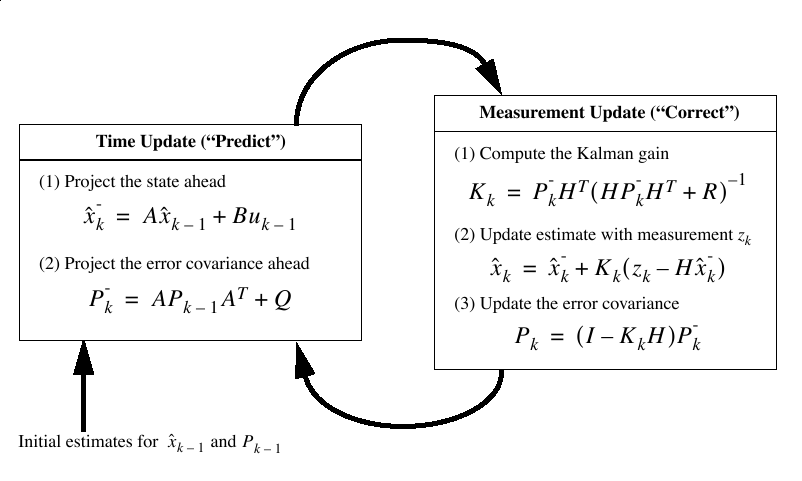
\includegraphics[scale=0.35]{../relazione/figure/cicloKalman.png}
\caption{\tiny \textit{Ciclo di Kalman completo}\label{fig:completeKalman}}
\end{figure}

}

\frame{\frametitle{Il Modello - 1}
Per descrivere il moto dei nostri oggetti ci è sembrata la scelta più semplice rappresentare il
generico moto di un punto nel piano.

\begin{figure}[hb]
\centering
	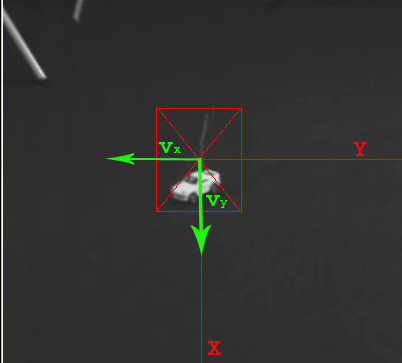
\includegraphics[scale=0.3]{../relazione/figure/motopiano.png}
\caption{\textit{Esempio di vettori di stato moto sul piano}\label{fig:motopiano}}
\end{figure}

\begin{footnotesize}
\begin{itemize}
\item $(x,y)$ è la posizione data secondo le coordinate 
\item $(v_x,v_y)$ è la velocità rispettivamente orizzontale e verticale dell'oggetto nel punto $(x,y)$ 
\end{itemize}
\end{footnotesize}
}


\frame{\frametitle{Il Modello - 2}
\begin{itemize}
\item \begin{math} x= \begin{bmatrix} x \\ y \\ v_{x} \\ v_{y} \end{bmatrix} \end{math}  \footnotesize{è il vettore di stato}\\
\end{itemize}

\begin{itemize}
\item $A = \begin{bmatrix} 1 & 0 & \Delta_{t} & 0 \\ 0 & 1 & 0 & \Delta_{t} \\ 0 & 0 & 1 & 0 \\ 0 & 0 & 0 & 1 \end{bmatrix}$ \footnotesize{è la matrice di transizione del modello}\\
\end{itemize}

\begin{itemize}
\item $B u_{t} = 0$ \footnotesize{sull'oggetto non agiscono forze esterne}
\end{itemize}
}

\frame{\frametitle{Il modello - 3}
\begin{columns}
\column{.50 \textwidth}
\begin{itemize}
\item $Q = \begin{bmatrix} \rho & 0 & 0 & 0 \\ 0 & \rho & 0 & 0 \\ 0 & 0 & \rho & 0 \\ 0 & 0 & 0 & \rho  \end{bmatrix}$ 
\end{itemize}
\column{.50 \textwidth}
\begin{footnotesize}covarianza del processo che rappresenta il rumore sul sistema\end{footnotesize}
\end{columns}

\begin{columns}
\column{.50 \textwidth}
\begin{itemize}
\item $H = \begin{bmatrix} 1 & 0 & 0 & 0 \\ 0 & 1 & 0 & 0 \end{bmatrix}$
\end{itemize}
\column{.50 \textwidth}
\begin{footnotesize}sceglie le componenti dello stato per confrontarlo con la misura\end{footnotesize}
\end{columns}

\begin{itemize}
\item $R = \begin{bmatrix} 0.285 & 0.005 \\ 0.005 & 0.046 \end{bmatrix}$ \begin{footnotesize}definisce il rumore associato alla misura\end{footnotesize}
\end{itemize}
}

\subsection{Condesation}

\frame{\frametitle{Condensation - 1}

E' un'implementazione del Particle Filter, un filtro di tipo Ricorsivo Bayesiano.

\begin{block}{Conditional Density Propagation}
\begin{itemize}
\item E' un algoritmo di tipo probabilistico che risulta molto robusto rispetto a dati rumorosi e a cambiamenti di stato non lineari.
 
\item Permette di essere utilizzato per lo studio di moti descritti anche da modelli complessi di tipo non lineare.

\item Supporta previsoni di tipo multimodale.

\item L'algoritmo utilizza un campionamento casuale e ordinato delle posizioni assunte dall'oggetto nei vari istanti di tempo per modellare funzioni di densità di probabilità arbitrariamente complesse.

\end{itemize}
\end{block}

}

\frame{\frametitle{Condensation - 2}

Utilizza un numero N finito di campioni per approssimare la curva che descrive la distribuzione dei dati $p(x_k \vline z_{1:k})$.\\~\\
Ciascun campione -  sample - consiste di due valori: lo stato e il peso.

\begin{block}{}
Chiamiamo con $H_{t}$ il vettore dei samples all'istante $t$:
\begin{center}
$H_t = \{\overrightarrow{s_1}(t), ... ,\overrightarrow{s_N}(t)\}$
\end{center}

Dove:
\begin{itemize}
\item $\overrightarrow{s_i}(t)= \{\overrightarrow{x_i}(t),p(x_i(t))\}$
\item $\overrightarrow{x_i}(t)$ è la posizione associata al sample $i$ all'istante $t$.
\item $p(\overrightarrow{x_i}(t))$ è la probabilità associata alla posizione $\overrightarrow{x_i}(t)$ che caratterizza il sample $i$
\end{itemize}
\end{block}

}

\frame{\frametitle{Algoritmo - Inizializzazione}
Al primo passo dell'algoritmo si inizializza tutti i samples:
\begin{itemize}
\item Ciascuna posizione può essere scelta in modo casuale secondo una distibuzione uniforme.
\item La probabilità associata a ciascun sample è invece distribuita secondo una gaussiana standard centrata nel valore medio tra il valore massimo e il valore minimo assumibile per la posizione dell'oggetto e la relativa varianza.
\end{itemize}

}


\frame{\frametitle{Algoritmo - passo t}

\begin{itemize}
\item Il sample $\overrightarrow{s_{\bar{i}}}(t)$ con probabilità maggiore è la predizione per il Condensation al passo t.\\
\end{itemize}

Per passare dal vettore $H_{t}$ al vettore $H_{t+1}$ si eseguono questi passi:
\begin{block}{}
\begin{small}
\begin{enumerate}
\item Si campiona la posizione reale dell'oggetto: $\overrightarrow{z}(t)$
\item Si calcola la posizione per ciascun sample secondo lo spostamento dato dal modello dinamico che descrive il moto dell'oggetto: 
\begin{equation}
	\overrightarrow{x_i}(t+1)= f(\overrightarrow{x_i}(t))
\end{equation}
\item Si stima la probabilità $p(\overrightarrow{z}(t))$ secondo la densità di probabilità dei campioni all'istante t centrata in $\overrightarrow{x_{\bar{i}}}(t)$.
\item Per ogni sample è ricalcolata la probabilità condizionata applicando il teorema di Bayes:
\begin{equation}
	p_i(\overrightarrow{x_i}(t+1))= p(\overrightarrow{x_i}(t)\ \mid \overrightarrow{z}(t))
\end{equation}
\end{enumerate}
\end{small}
\end{block}

}


\frame{\frametitle{Il Modello - 4}
La nostra implementazione del Condensation rispetta fedelmete l'algoritmo che è stato prima presentato.\\~\\
Per quanto riguarda il modello dinamico associato si è utilizzata la stessa equazione valida per il tracciamento fatto con il filtro di Kalman:
\begin{block}{}
\begin{small}
\begin{equation}
x_{t+1} = A  x_t
\end{equation}
Dove:
\begin{center}
$A = \begin{bmatrix} 1 & 0 & \Delta_{t} & 0 \\ 0 & 1 & 0 & \Delta_{t} \\ 0 & 0 & 1 & 0 \\ 0 & 0 & 0 & 1 \end{bmatrix} $
\end{center}
\end{small}
\end{block}

}


%%%PARTE DI MEO %%%
%%%%%%%%%%%%%%%%%%%%%%%%%%%%%%%%%%%%%%%%%%
\section{Esperimenti}
\frame{\frametitle{Ciclo di lavoro}
\centering
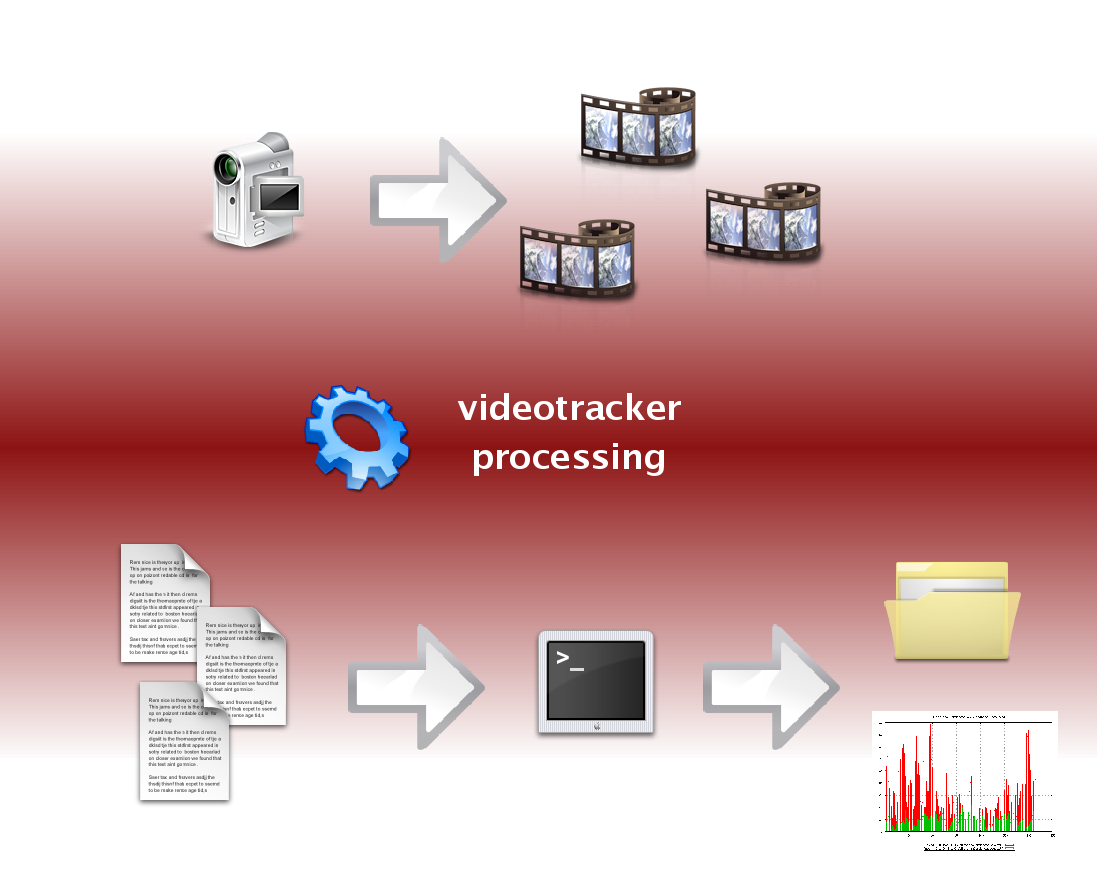
\includegraphics[scale=0.35]{img/Presentazione.png}

}

%%%%%%%%%%%%%%%%%%%%%%%%%%%%%%%%%%%%%%%%%%
\frame{\frametitle{Parametri degli esperimenti}
\begin{block}{}\begin{small}\alert{\textbf{Esperimenti}}: variazione di tre parametri nei tre video selezionati \end{small}\end{block}
\pause
\begin{footnotesize}\begin{description}
\item [\textbf{Intervallo Frames}] Frames tra due applicazioni consecutive del Tracking\\Allontanamento dalle condizioni ottimali di lavoro, simulazione del comportamento dei tracker reali. \pause
\item [\textbf{Q - Area Kalman}] Autovalori della matrice del rumore sul processo (Q)\\Ririsulta l'area di confidenza del filtro di \alert{Kalman}, ovvero l'area nella quale deve risiedere il blob al frame precedente per poter continuare ad essere tracciato all'esecuzione successiva.\pause
\item [\textbf{Samples ConDensation}] Numero dei samples ad ogni esecuzione\\ \`E il numero totale di samples che utilizza il \alert{ConDensation} per effettuare i calcoli statistici ad ogni esecuzione del Tracking
 \end{description}\end{footnotesize}

}
%%%%%%%%%%%%%%%%%%%%%%%%%%%%%%%%%%%%%%%%%%
\frame{\frametitle{Output \& Scripting}
\begin{block}{}
\begin{small}Il software produce sei files di output:\end{small}
\begin{scriptsize}\begin{description}
\item [\textit{coordinateReali.txt}] Coordinate reali dell'oggetto da tracciare
\item [\textit{coordinateKalman.txt}] Coordinate previste da Kalman
\item [\textit{coordinateCondensation.txt}] Coordinate previste dal ConDensation
\item [\textit{distanzaKalman.txt}] \alert{$\delta_k$} Distanza tra le coordinate reali e la previsione di Kalman
\item [\textit{distanzaCondensation.txt}]\alert{$\delta_c$} Distanza tra coord reali e previsione ConDensation
\item [\textit{Risultati.txt~~~~~~~~~~~}]  distanza media, $\overline{\delta}_k, \overline{\delta}_c$, varianza media ConDensation ($\overline{\sigma}_x, \overline{\sigma}_y$).
 \end{description}\end{scriptsize}
\end{block}
\pause
\begin{small}I files ottenuti vengono processati da due \alert{script bash}\end{small}
\begin{scriptsize}\begin{description}
\item [\textbf{gplot.sh}] Invoca degli script \alert{GNUPlot} che restituiscono dei grafici relativi ai risultati ottenuti, consentendo una valutazione immediata dell'esperimento effettuato.
\item[\textbf{exp.sh}] Organizza i files di output e le immagini comparative disegnate nel filesystem, consentendo un facile \alert{riepilogo} dei risultati ed una ordinata catalogazione di questi.
 \end{description}\end{scriptsize}
}
%%%%%%%%%%%%%%%%%%%%%%%%%%%%%%%%%%%%%%%%%%
\subsection{Video}

\frame{\frametitle{Video selezionati}
\hrulefill
\begin{columns}
\column{.30\textwidth}\centering
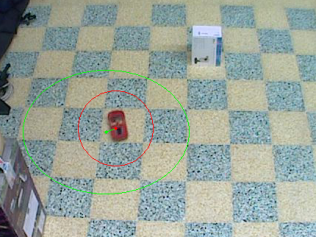
\includegraphics[scale=0.21]{img/movie12.png}

\column{.70\textwidth}
\begin{footnotesize}\begin{enumerate}
\item [1] \textbf{movie12.mjpeg} (mjpeg/xvid)
	\begin{itemize}
	\item[-] occlusione, moto circolare e costante
	\item[-] 640x480, 25$fps$, 50.4$s$\end{itemize}
\end{enumerate}\end{footnotesize}
\end{columns}

\hrulefill \pause

\begin{columns}
\column{.70\textwidth}
\begin{footnotesize}\begin{enumerate}
\item[2] \textbf{tappeto\_nozoom.avi} (avi/xvid)
	\begin{itemize}
	\item[-] moto vario, repentine accelerazioni, oggetto entra ed esce dalla scena
	\item[-] 320x240, 10$fps$, 59$s$\end{itemize}
\end{enumerate}\end{footnotesize}
\column{.30\textwidth}\centering
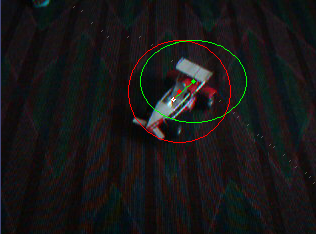
\includegraphics[scale=0.21]{img/tappetonozoom.png}
\end{columns}

\hrulefill \pause

\begin{columns}
\column{.30\textwidth}\centering
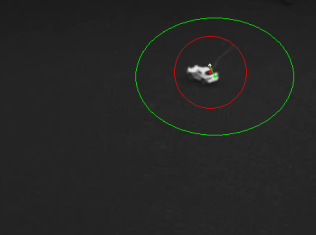
\includegraphics[scale=0.21]{img/singlecar.png}
\column{.70\textwidth}
\begin{footnotesize}\begin{enumerate}
\item[3] \textbf{singlecar.avi} (avi/xvid)
	\begin{itemize}
	\item[-] moto costante, oggetto entra ed esce dalla scena
	\item[-] 648x484, 30$fps$, 33$s$\end{itemize}
\end{enumerate}\end{footnotesize}
\end{columns}
\hrulefill
}


% \frame{\frametitle{Primo video - movie12.mjpeg}
% \begin{columns}
% \column{.65\textwidth}
% \begin{small}\begin{itemize}
%  \item occlusione, moto circolare e costante
% \item 640x480, 25$fps$, 50.4$s$
% \end{itemize}\end{small}
% 
% \column{.35\textwidth}\centering
% 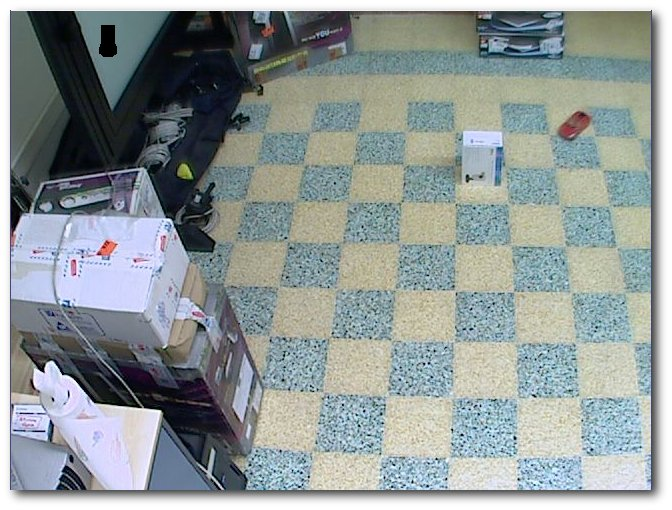
\includegraphics[scale=0.15]{../relazione/figure/movie12.jpg}
% \end{columns}
% \begin{columns}
% 
% \column{.20\textwidth}
% \begin{scriptsize}
% \begin{itemize}
% \item [M]3
% \item [Q]1000
% \item [S]1000
% \end{itemize}
% \end{scriptsize}
% 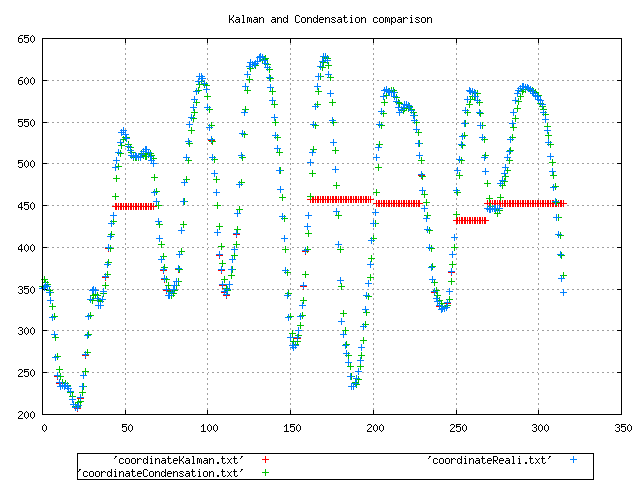
\includegraphics[scale=0.1]{../esperimenti/movie12/mod_3-Q_1000-S_1000/plot.png}\\
% 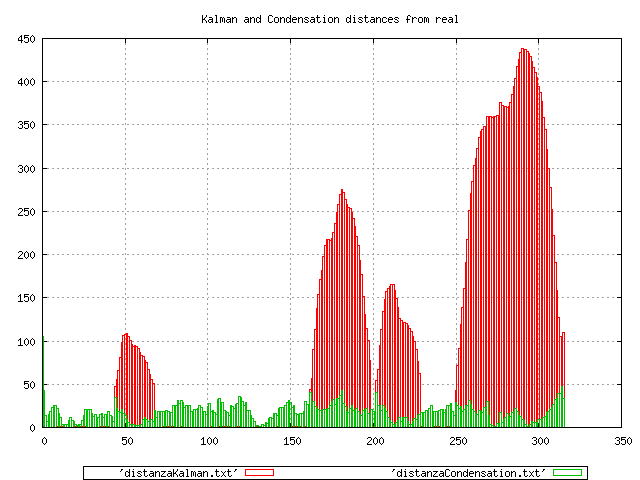
\includegraphics[scale=0.1]{../esperimenti/movie12/mod_3-Q_1000-S_1000/plot-distances.png}
% 
% \column{.20\textwidth}
% \begin{scriptsize}
% \begin{itemize}
% \item [M]3
% \item [Q]2000
% \item [S]1000
% \end{itemize}
% \end{scriptsize}
% 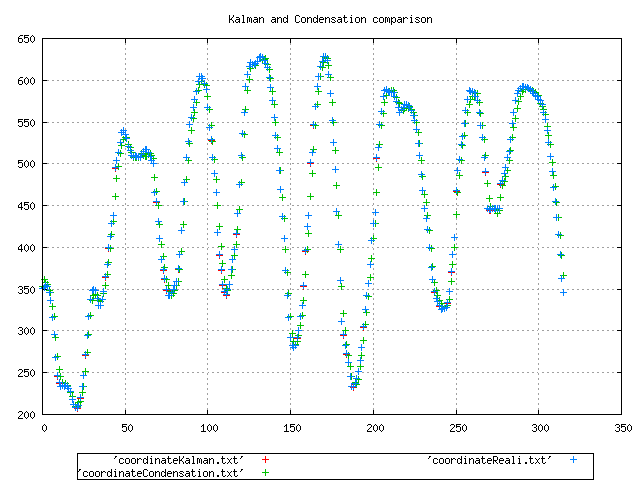
\includegraphics[scale=0.1]{../esperimenti/movie12/mod_3-Q_2000-S_1000/plot.png}\\
% 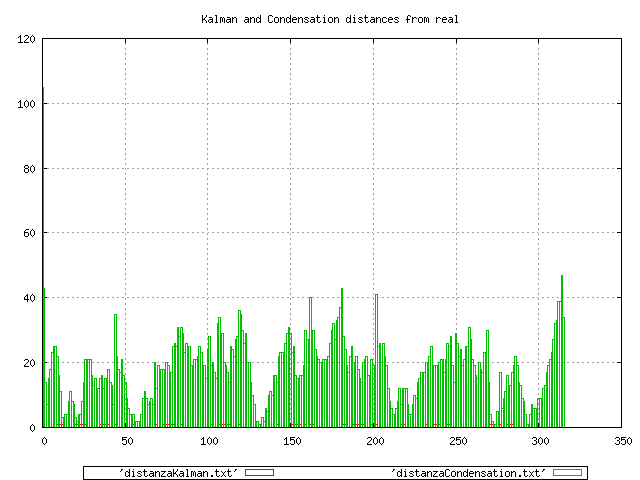
\includegraphics[scale=0.1]{../esperimenti/movie12/mod_3-Q_2000-S_1000/plot-distances.png}
% 
% \column{.20\textwidth}
% \begin{scriptsize}
% \begin{itemize}
% \item [M]3
% \item [Q]1000
% \item [S]5000
% \end{itemize}
% \end{scriptsize}
% 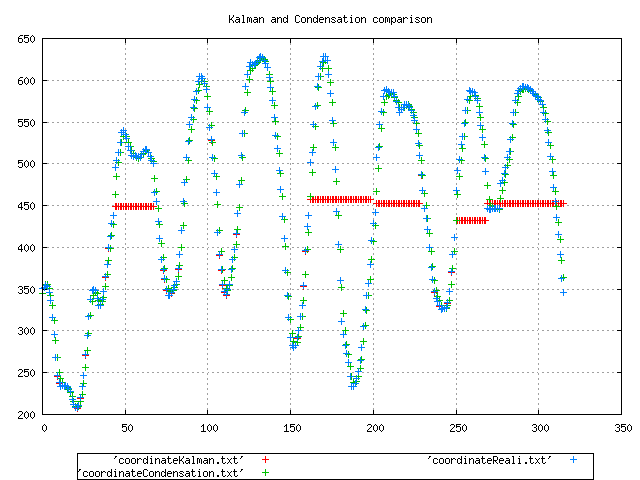
\includegraphics[scale=0.1]{../esperimenti/movie12/mod_3-Q_1000-S_5000/plot.png}\\
% 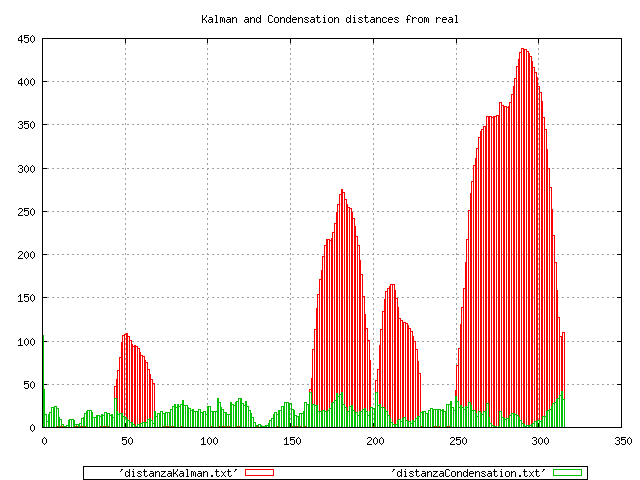
\includegraphics[scale=0.1]{../esperimenti/movie12/mod_3-Q_1000-S_5000/plot-distances.png}
% 
% \column{.20\textwidth}
% \begin{scriptsize}
% \begin{itemize}
% \item [M]3
% \item [Q]1000
% \item [S]100
% \end{itemize}
% \end{scriptsize}
% 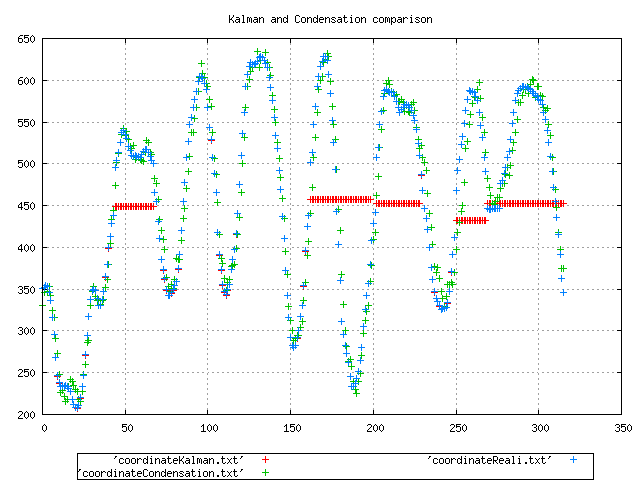
\includegraphics[scale=0.1]{../esperimenti/movie12/mod_3-Q_1000-S_100/plot.png}\\
% 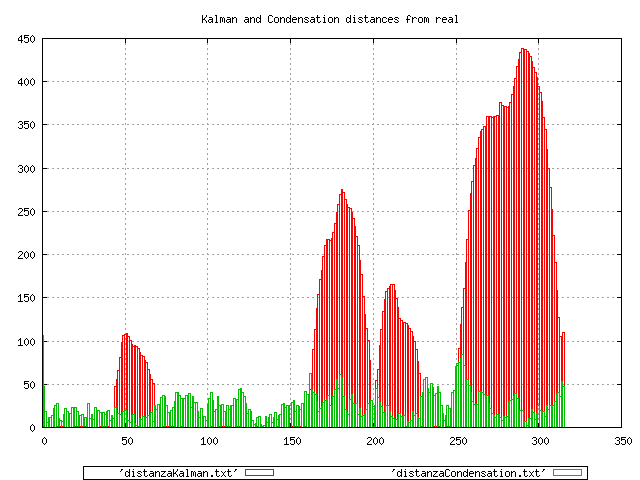
\includegraphics[scale=0.1]{../esperimenti/movie12/mod_3-Q_1000-S_100/plot-distances.png}
% \end{columns}
% 
% }
% %%%%%%%%%%%%%%%%%%%%%%%%%%%%%%%%%%%%%%%%%%
% \frame{\frametitle{Secondo video - tappetonozoom.avi}
% \begin{columns}
% \column{.65\textwidth}
% \begin{small}\begin{itemize}
%  \item moto vario, repentine accelerazioni, oggetto entra ed esce dalla scena
% \item 320x240, 10$fps$, 59$s$
% \end{itemize}\end{small}
% 
% \column{.35\textwidth}\centering
% 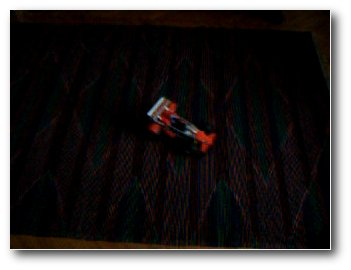
\includegraphics[scale=0.25]{../relazione/figure/tappeto_nozoom.jpg}
% \end{columns}
% \begin{columns}
% 
% \column{.20\textwidth}
% \begin{scriptsize}
% \begin{itemize}
% \item [M]3
% \item [Q]1000
% \item [S]1000
% \end{itemize}
% \end{scriptsize}
% 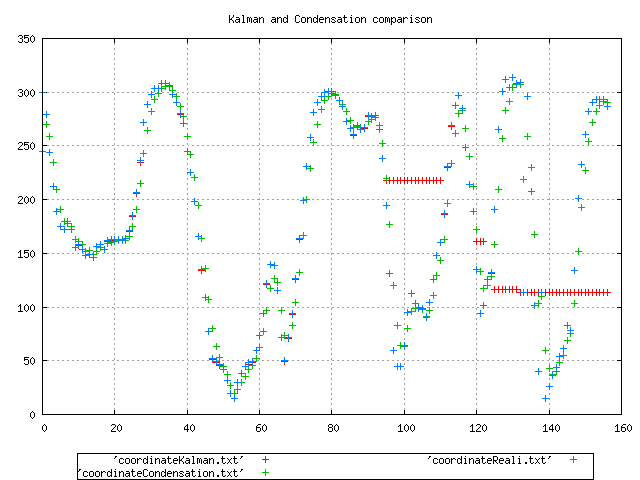
\includegraphics[scale=0.1]{../esperimenti/tappeto_nozoom/mod_3-Q_1000-S_1000/plot.png}\\
% 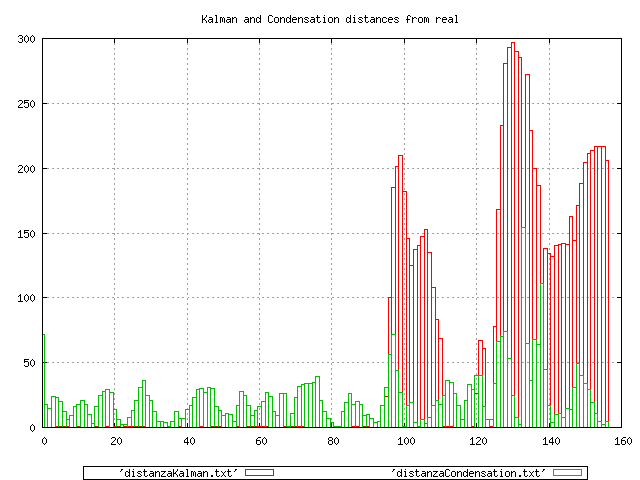
\includegraphics[scale=0.1]{../esperimenti/tappeto_nozoom/mod_3-Q_1000-S_1000/plot-distances.png}
% 
% \column{.20\textwidth}
% \begin{scriptsize}
% \begin{itemize}
% \item [M]5
% \item [Q]1000
% \item [S]1000
% \end{itemize}
% \end{scriptsize}
% 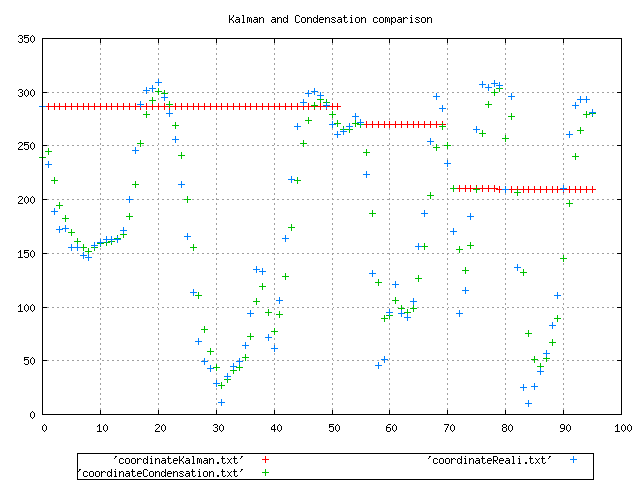
\includegraphics[scale=0.1]{../esperimenti/tappeto_nozoom/mod_5-Q_1000-S_1000/plot.png}\\
% 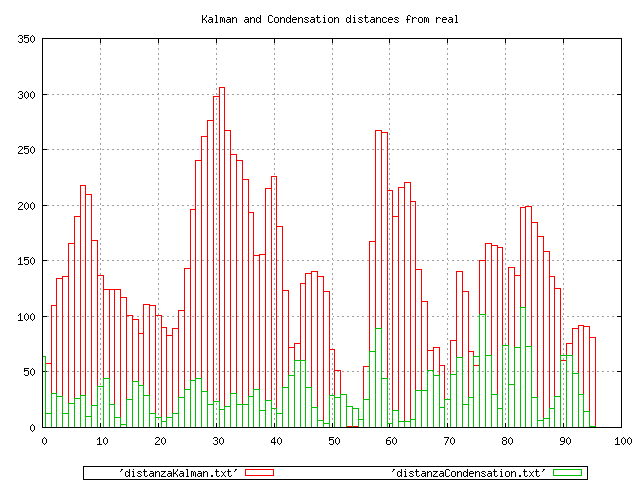
\includegraphics[scale=0.1]{../esperimenti/tappeto_nozoom/mod_5-Q_1000-S_1000/plot-distances.png}
% 
% 
% \column{.20\textwidth}
% \begin{scriptsize}
% \begin{itemize}
% \item [M]2
% \item [Q]1000
% \item [S]1000
% \end{itemize}
% \end{scriptsize}
% 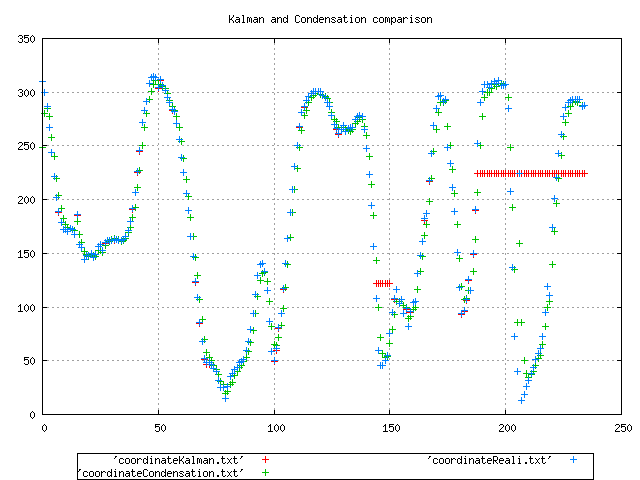
\includegraphics[scale=0.1]{../esperimenti/tappeto_nozoom/mod_2-Q_1000-S_1000/plot.png}\\
% 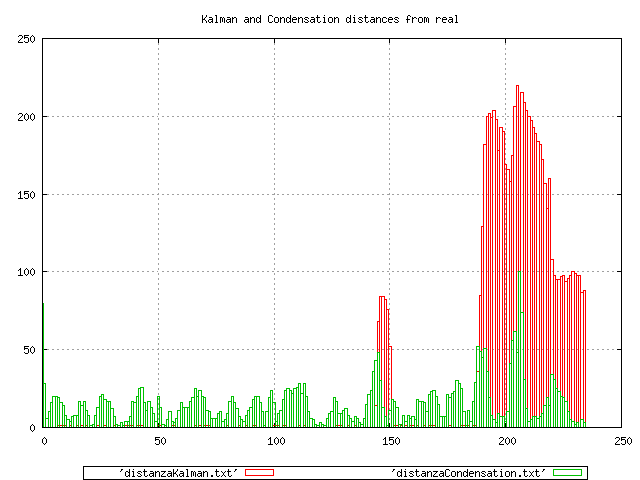
\includegraphics[scale=0.1]{../esperimenti/tappeto_nozoom/mod_2-Q_1000-S_1000/plot-distances.png}
% 
% 
% \column{.20\textwidth}
% \begin{scriptsize}
% \begin{itemize}
% \item [M]1
% \item [Q]2000
% \item [S]1000
% \end{itemize}
% \end{scriptsize}
% 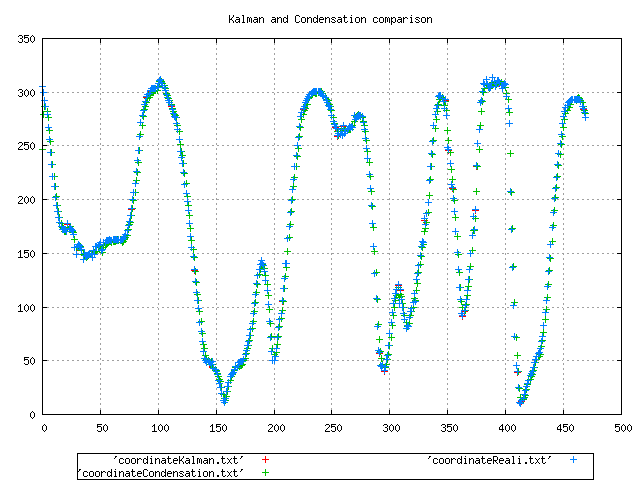
\includegraphics[scale=0.1]{../esperimenti/tappeto_nozoom/mod_1-Q_2000-S_1000/plot.png}\\
% 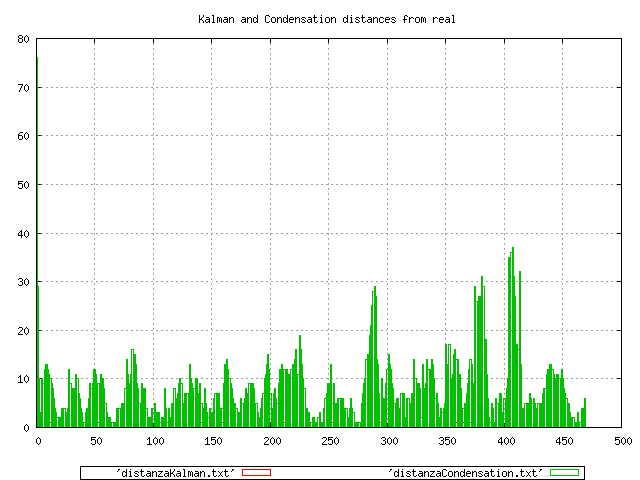
\includegraphics[scale=0.1]{../esperimenti/tappeto_nozoom/mod_1-Q_2000-S_1000/plot-distances.png}
% \end{columns}
% 
% }
% %%%%%%%%%%%%%%%%%%%%%%%%%%%%%%%%%%%%%%%%%%
% \frame{\frametitle{Terzo video - singlecar.avi}
% \begin{columns}
% \column{.65\textwidth}
% \begin{small}\begin{itemize}
%  \item moto costante, oggetto entra ed esce dalla scena
% \item 648x484, 30$fps$, 33$s$
% \end{itemize}\end{small}
% 
% \column{.35\textwidth}\centering
% 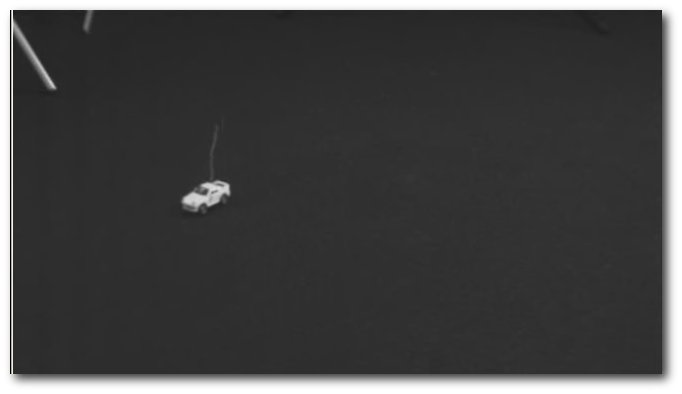
\includegraphics[scale=0.15]{../relazione/figure/singlecar.jpg}
% \end{columns}
% \begin{columns}
% 
% \column{.20\textwidth}
% \begin{scriptsize}
% \begin{itemize}
% \item [M]3
% \item [Q]1000
% \item [S]1000
% \end{itemize}
% \end{scriptsize}
% 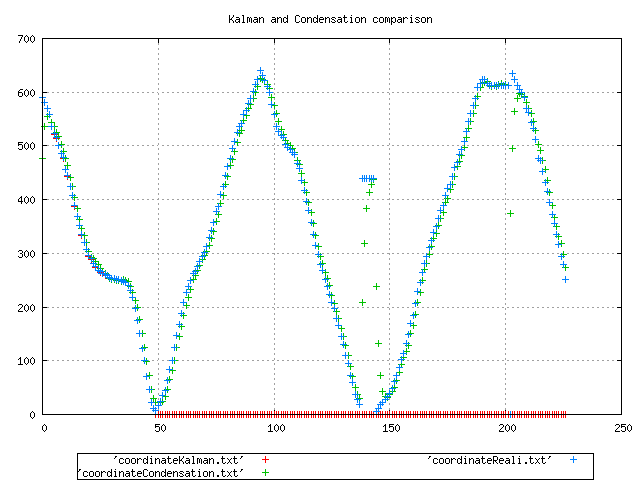
\includegraphics[scale=0.1]{../esperimenti/single_car/mod_3-Q_1000-S_1000/plot.png}\\
% 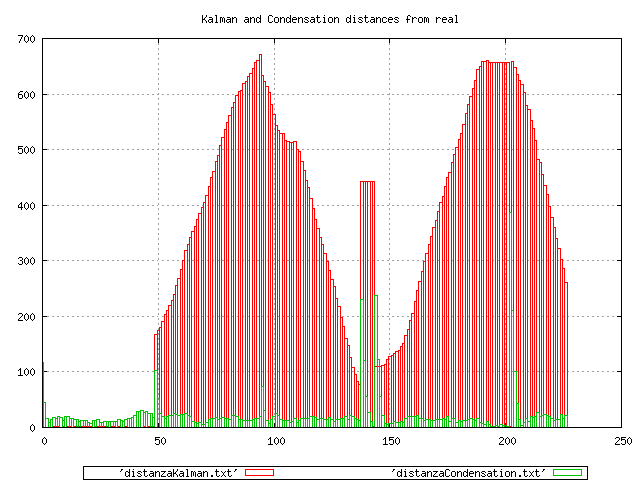
\includegraphics[scale=0.1]{../esperimenti/single_car/mod_3-Q_1000-S_1000/plot-distances.png}
% 
% \column{.20\textwidth}
% \begin{scriptsize}
% \begin{itemize}
% \item [M]10
% \item [Q]5000
% \item [S]1000
% \end{itemize}
% \end{scriptsize}
% 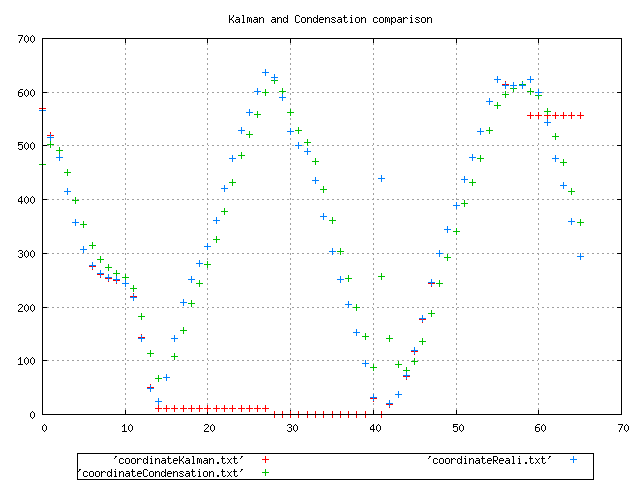
\includegraphics[scale=0.1]{../esperimenti/single_car/mod_10-Q_5000-S_1000/plot.png}\\
% 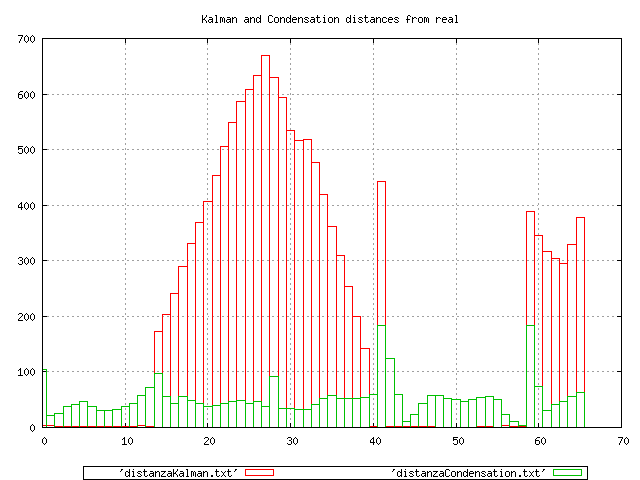
\includegraphics[scale=0.1]{../esperimenti/single_car/mod_10-Q_5000-S_1000/plot-distances.png}
% 
% \column{.20\textwidth}
% \begin{scriptsize}
% \begin{itemize}
% \item [M]6
% \item [Q]0.1
% \item [S]1000
% \end{itemize}
% \end{scriptsize}
% 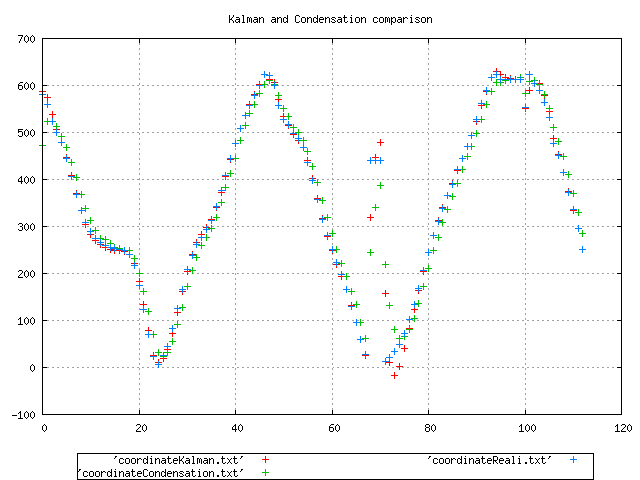
\includegraphics[scale=0.1]{../esperimenti/single_car/mod_6-Q_0.1-S_1000/plot.png}\\
% 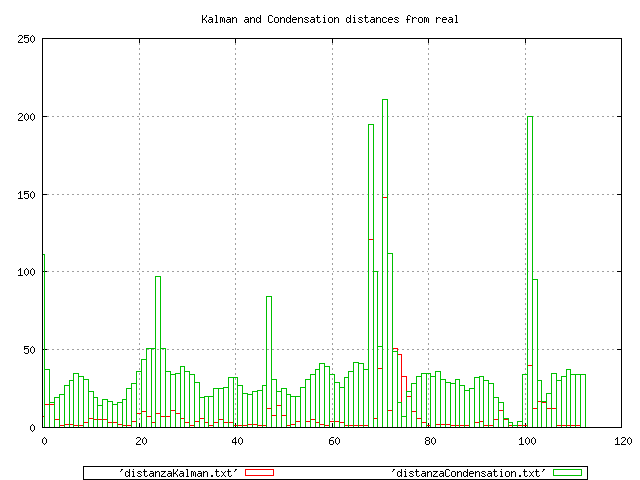
\includegraphics[scale=0.1]{../esperimenti/single_car/mod_6-Q_0.1-S_1000/plot-distances.png}
% 
% \column{.20\textwidth}
% \begin{scriptsize}
% \begin{itemize}
% \item [M]1
% \item [Q]0.0001
% \item [S]1000
% \end{itemize}
% \end{scriptsize}
% 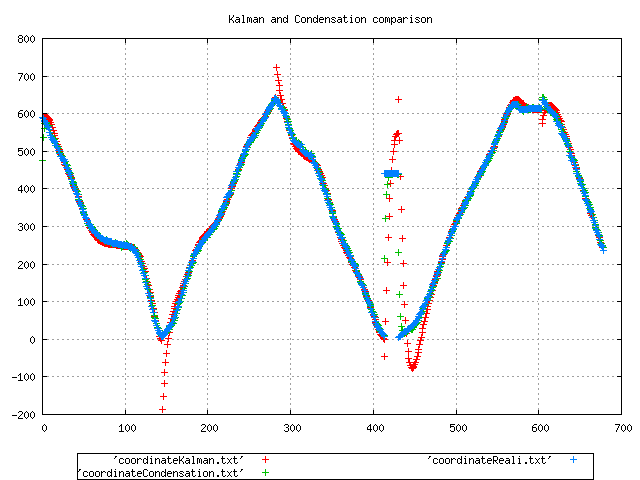
\includegraphics[scale=0.1]{../esperimenti/single_car/mod_1-Q_0.0001-S_1000/plot.png}\\
% 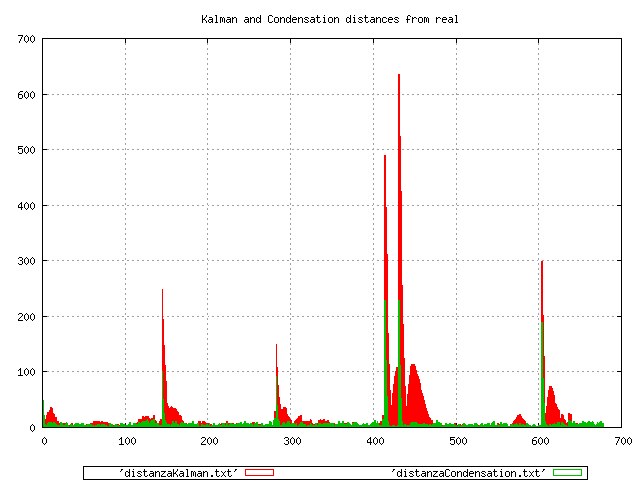
\includegraphics[scale=0.1]{../esperimenti/single_car/mod_1-Q_0.0001-S_1000/plot-distances.png}
% \end{columns}
% }
%%%%%%%%%%%%%%%%%%%%%%%%%%%%%%%%%%%%%%%%%%
\subsection{Risultati}

%%%%%%%%%%%%%%%%%%%%%%%%%%%%%%%%%%%%%%%%%%
\frame{\frametitle{movie12.mjpeg - MOD:3, Q:1000, S:1000}

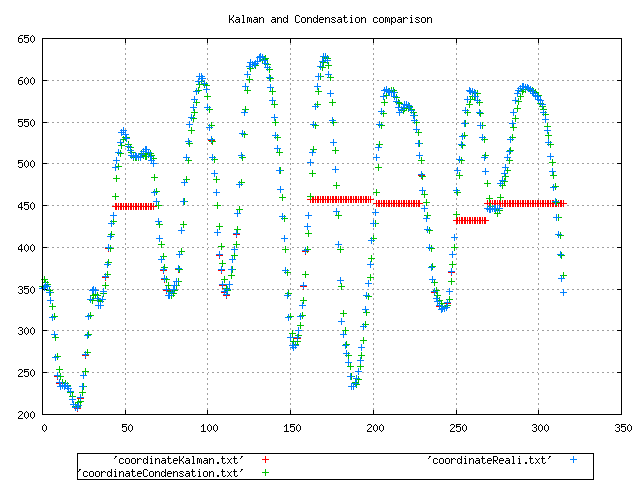
\includegraphics[scale=0.45]{../esperimenti/movie12/mod_3-Q_1000-S_1000/plot.png}

}
%%%%%%%%%%%%%%%%%%%%%%%%%%%%%%%%%%%%%%%%%%
\frame{\frametitle{movie12.mjpeg - MOD:3, Q:1000, S:10}
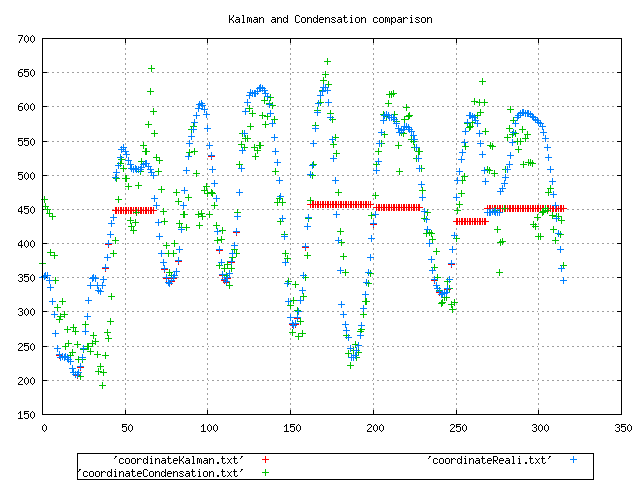
\includegraphics[scale=0.45]{../esperimenti/movie12/mod_3-Q_1000-S_10/plot.png}
}
%%%%%%%%%%%%%%%%%%%%%%%%%%%%%%%%%%%%%%%%%%
\frame{\frametitle{movie12.mjpeg - MOD:3, Q:1000, S:1000}
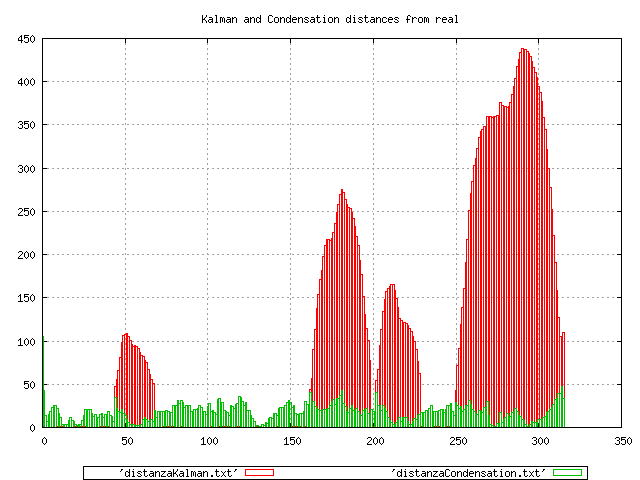
\includegraphics[scale=0.45]{../esperimenti/movie12/mod_3-Q_1000-S_1000/plot-distances.png}
}
%%%%%%%%%%%%%%%%%%%%%%%%%%%%%%%%%%%%%%%%%%
\frame{\frametitle{movie12.mjpeg - MOD:3, Q:1000, S:10}
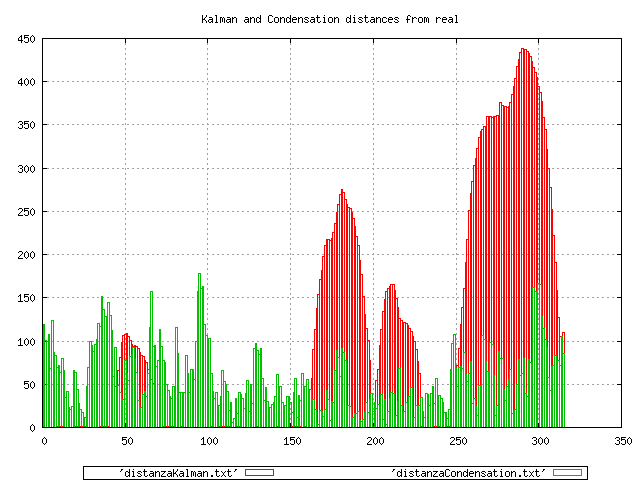
\includegraphics[scale=0.45]{../esperimenti/movie12/mod_3-Q_1000-S_10/plot-distances.png}
}


% 
%%%%%%%%%%%%%%%%%%%%%%%%%%%%%%%%%%%%%%%%%%
\frame{\frametitle{tappetonozoom.avi - MOD:2, Q:1000, S:1000}
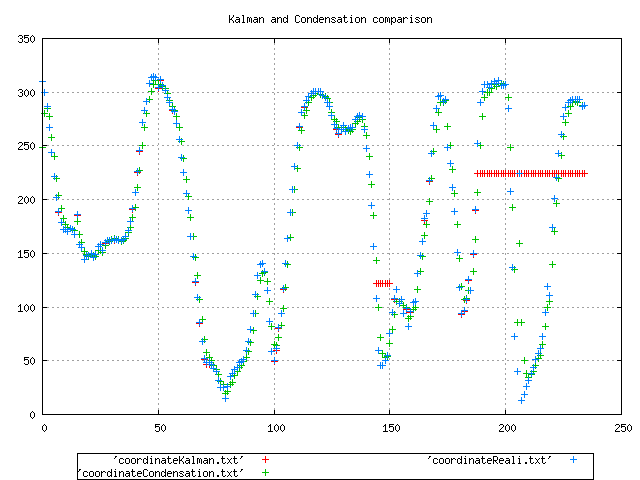
\includegraphics[scale=0.45]{../esperimenti/tappeto_nozoom/mod_2-Q_1000-S_1000/plot.png}
}
%%%%%%%%%%%%%%%%%%%%%%%%%%%%%%%%%%%%%%%%%%
\frame{\frametitle{tappetonozoom.avi - MOD:1, Q:500, S:10}
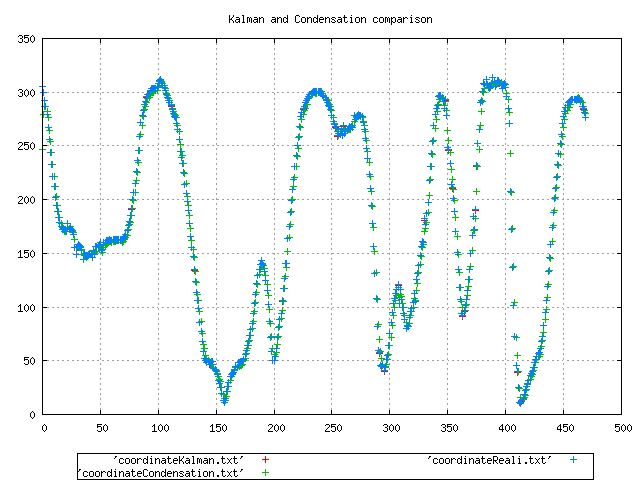
\includegraphics[scale=0.45]{../esperimenti/tappeto_nozoom/mod_1-Q_500-S_1000/plot.png}
}
%%%%%%%%%%%%%%%%%%%%%%%%%%%%%%%%%%%%%%%%%%
\frame{\frametitle{tappetonozoom.avi - MOD:2, Q:1000, S:1000}
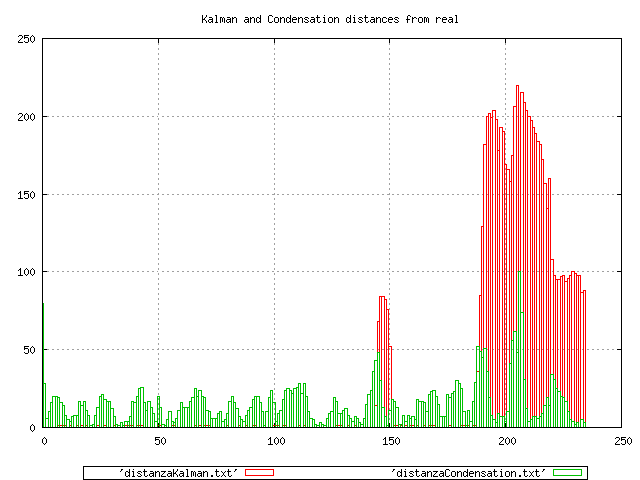
\includegraphics[scale=0.45]{../esperimenti/tappeto_nozoom/mod_2-Q_1000-S_1000/plot-distances.png}
}
%%%%%%%%%%%%%%%%%%%%%%%%%%%%%%%%%%%%%%%%%%
\frame{\frametitle{tappetonozoom.avi - MOD:1, Q:500, S:10}
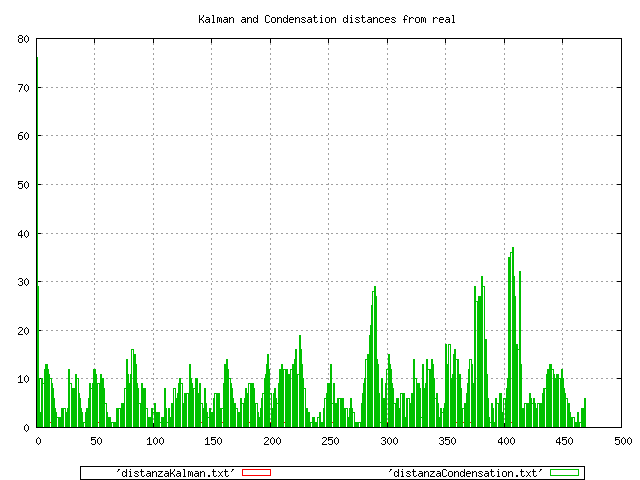
\includegraphics[scale=0.45]{../esperimenti/tappeto_nozoom/mod_1-Q_500-S_1000/plot-distances.png}
}


% 
%%%%%%%%%%%%%%%%%%%%%%%%%%%%%%%%%%%%%%%%%%
\frame{\frametitle{tappetonozoom.avi - MOD:1, Q:1, S:1000}
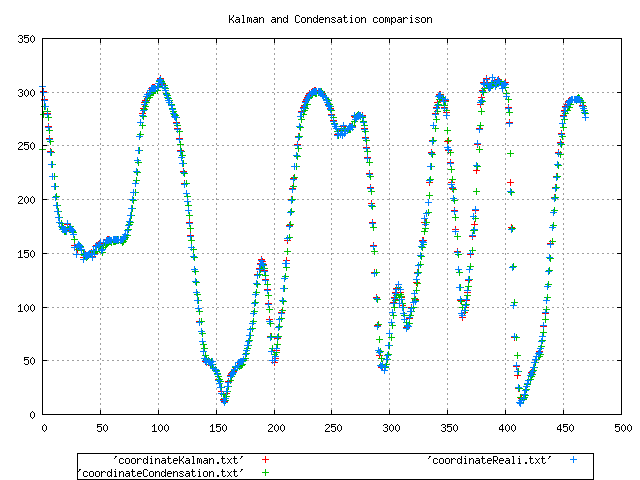
\includegraphics[scale=0.45]{../esperimenti/tappeto_nozoom/mod_1-Q_1-S_1000/plot.png}
}
%%%%%%%%%%%%%%%%%%%%%%%%%%%%%%%%%%%%%%%%%%
\frame{\frametitle{tappetonozoom.avi - MOD:1, Q:0.001, S:1000}
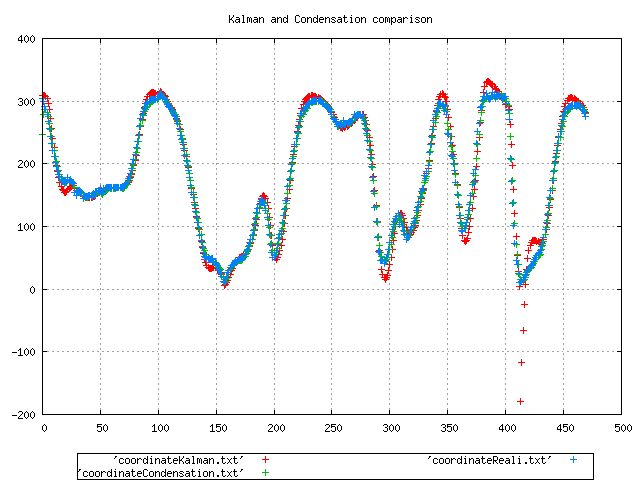
\includegraphics[scale=0.45]{../esperimenti/tappeto_nozoom/mod_1-Q_0.001-S_1000/plot.png}
}
%%%%%%%%%%%%%%%%%%%%%%%%%%%%%%%%%%%%%%%%%%
\frame{\frametitle{tappetonozoom.avi - MOD:1, Q:1, S:1000}
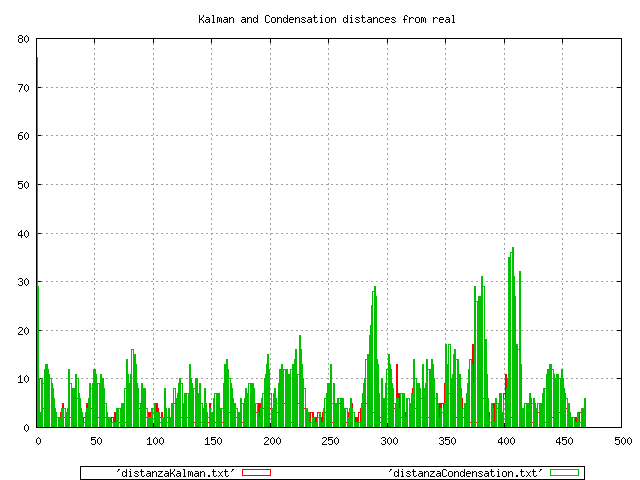
\includegraphics[scale=0.45]{../esperimenti/tappeto_nozoom/mod_1-Q_1-S_1000/plot-distances.png}
}
%%%%%%%%%%%%%%%%%%%%%%%%%%%%%%%%%%%%%%%%%%
\frame{\frametitle{tappetonozoom.avi - MOD:1, Q:0.001, S:1000}
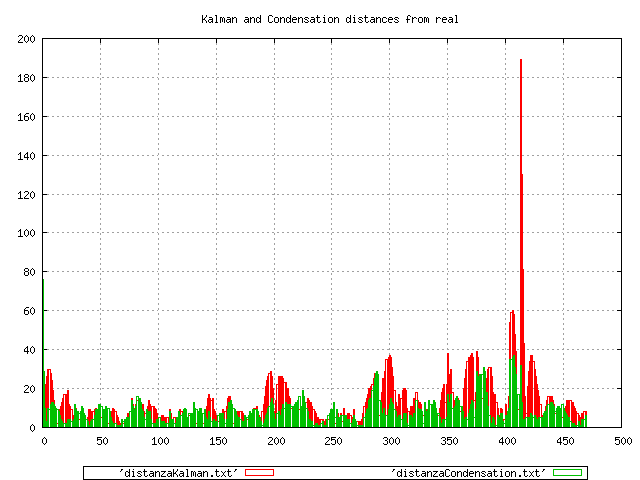
\includegraphics[scale=0.45]{../esperimenti/tappeto_nozoom/mod_1-Q_0.001-S_1000/plot-distances.png}
}

%%%Conclusione %%%
%%%%%%%%%%%%%%%%%%%%%%%%%%%%%%%%%%%%%%%%%%
\section{Conclusione}
%%%%%%%%%%%%%%%%%%%%%%%%%%%%%%%%%%%%%%%%%
\frame{\frametitle{Conclusione}

\textcolor{UNL@Scarlet}{Filtro di Kalman}
\begin{itemize}
 \item Ottimo se eseguito ogni frame
\item Perde l'oggetto se fuori dall'area di confidenza
\item Impreciso su movimenti \textbf{non lineari}
\item Tentativo di predizione dell'oggetto non tracciato in caso di \textbf{occlusione}


\end{itemize}
\pause
\textcolor{UNL@Scarlet}{ConDensation}
\begin{itemize}
 \item Meno preciso di Kalman
\item Non perde mai l'oggetto
\item Efficiente su tracking \textbf{non lineare}
\item Ottimo tracciamento in caso di \textbf{occlusione}
\end{itemize}
\pause
\begin{block}{}
Non è possibile elevare uno dei due approcci come \alert{migliore}.\\
\alert{Tuning} dei parametri porta a conclusioni particolari.
\end{block}
}

%%%%%%%%%%%%%%%%%%%%%%%%%%%%%%%%%%%%%%%%%
\frame{\frametitle{Conclusione}

Materiale: software, risultati, relazione, presentazione
\begin{itemize}
 \item Rilasciato con licenza GPL
\item Disponibile su spazio SVN Google Code
	\\ \begin{tiny}svn checkout http://video-tracker.googlecode.com/svn/trunk/ video-tracker\end{tiny}
\item Sviluppato e testato sui sistemi operativi:
\begin{itemize}
\item []
\includegraphics[width=13pt]{img/UbuntuLogo.jpg}~Ubuntu/Kubuntu  6.10/7.04 
\item []
\includegraphics[width=13pt]{img/Windows.jpg}~Microsoft Windows XP
\end{itemize}

\item Video utilizzati:
\begin{itemize}
 \item Centro d'eccellenza \textbf{MICC} (Università di Firenze)
\item Produzione autonoma 
\end{itemize}

\end{itemize}
\pause
\begin{block}{}
\begin{center}
\textcolor{UNL@Scarlet}{http://code.google.com/p/video-tracker/}\end{center}\end{block}
}
%%%%%%%%%%%%%%%%%%%%%%%%%%%%%%%%%%%%%%%%%

\frame{\setbeamercolor{titlelike}{bg=UNL@Scarlet,fg=UNL@Cream}
\vspace{-10pt}
\begin{center}
\begin{scriptsize}
	\textsc{Università degli studi di Firenze}
\end{scriptsize}\\ 
\begin{tiny}
	Facoltà di Ingegneria - Corso di laurea specialistica in \textsc{Ingegneria Informatica}
\vspace{-20pt}
\end{tiny}
\end{center}

\titlepage
 }




\end{document}


